\section{Zielsetzung}
\label{sec:Zielsetzung}
Wird eine Oberfläche eines zu untersuchenden Materials Röntgenstrahlung ausgesetzt, wird ein Teil der Strahlung reflektiert. Die Intensität der reflektierten 
Strahlung lässt sich messen. Sind auch der Einfalls- und Ausfallswinkel bekannt, kann so eine Aussage über verschiedene Eigenschaften des Materials getroffen werden.
Ziel dieses Versuchs ist es, mithilfe der Röntenreflektometrie die Dichte, Rauigkeit und Dicke eines Polysterolfilms auf einem Siliziumwafer zu bestimmen.

\section{Theorie}
\label{sec:Theorie}
Als Röntgenstrahlung wird elektromagnetische Strahlung bezeichnet, die in einem Wellenlängenbereich von $\lambda = \qty{10}{\nano\metre}$ bis $\qty{10}{\pico\metre}$
liegt, was einer Energie von rund $\qty{100}{\eV}$ bis $\qty{150}{\kilo\eV}$ entspricht. Wie auch andere elektromagnetische Strahlung wird Röntgenstrahlung 
an einer Grenzfläche zu einem Teil reflektiert, während der andere Teil in das Material eindringt und dort unter Berücksichtigung der neuen Materialeigenschaften
propagiert.

\subsection{Erzeugung von Röntgenstrahlung}
Röntgenstrahlen sind nach ihrem Entdecker Wilhelm Conrad Röntgen benannt, der diese im Jahr 1895 erstmals künstlich erzeugte und ihre Eingenschaften untersuchte.

Eine der Möglichkeiten, Röntgenstrahlung zu erzeugen ist das Abbremsen von Elektronen in einem Anodenmaterial.
Dazu wird zunächst an eine Glühkathode eine Heizspannung angelegt, sodass aufgrund des glühelektrischen Effekts Elektronen aus dem Kathodenmaterial austreten.
Mittels einer angelegten Beschleunigungsspannug werden die freien Elektronen zu einer Anode hin beschleunigt. In dem Anodenmaterial werden die Elektronen stark in
dem Coulombfeld der Anodenatome abgebremst, wobei ein kontinuierliches Spektrum an Bremstrahlung abgestrahlt wird. 
Durch das Herauslösen von Elektronen der unteren Energieniveaus kommt es durch das Auffüllen dieser zur Emission von einer charakteristischen Strahlung, welche
materialabhängig und für die einzelnen Übergänge diskret ist.
Der schematische Aufbau einer Röntgenröhre ist in \autoref{fig:Röntgenröhre} gezeigt.

\begin{figure}
    \centering
    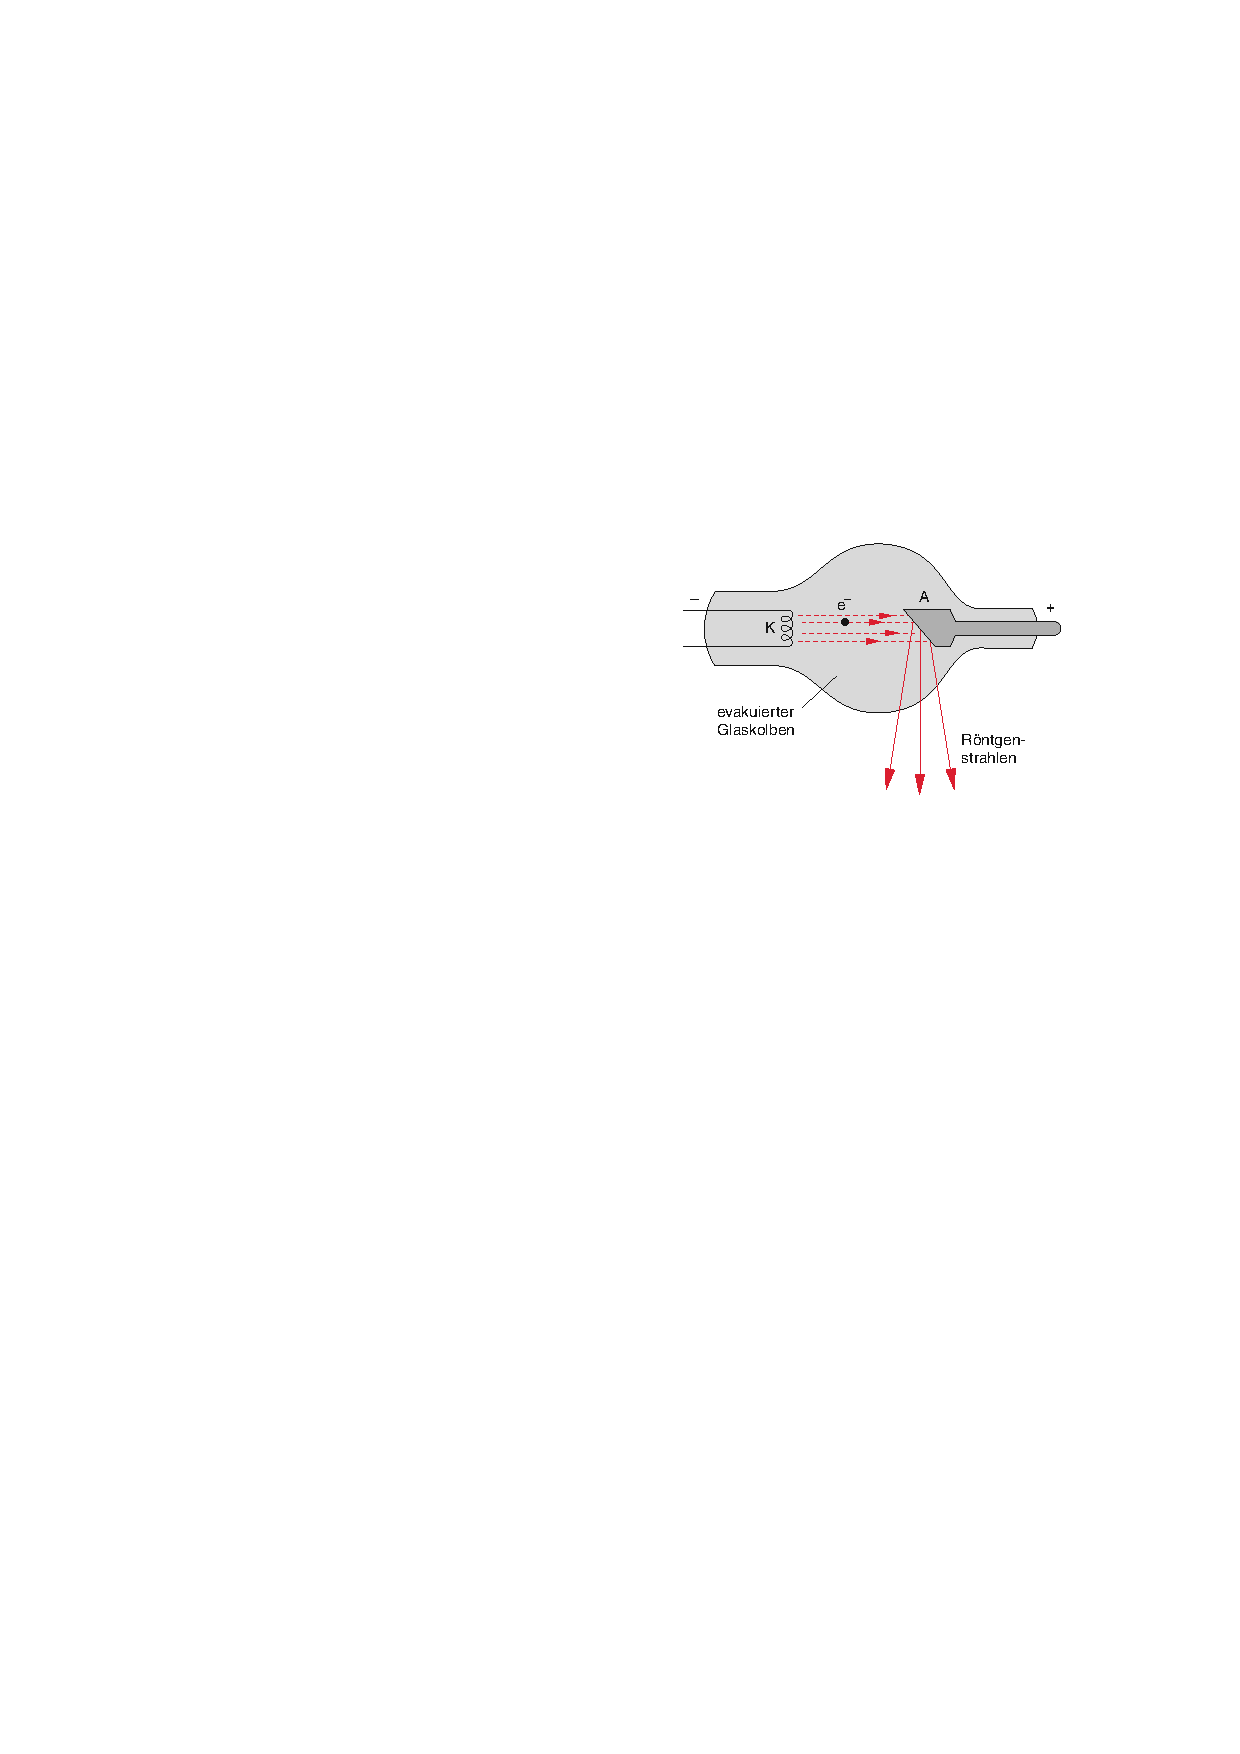
\includegraphics[width=0.5\textwidth]{content/pics/Röntgenröhre.pdf}
    \caption{Exemplarischer Aufbau einer Röntgenröhre. Aufgrund der thermischen Elektronenemission treten Elektronen aus der Glühkathode aus. %
    Diese werden im elektrischen Feld zwischen Kathode und Anode zur letzteren hin beschleunigt. In dem Anodenmaterial werden die Elektronen abgebremst und %
    Röntgenstrahlung wird emittiert \cite{Demtröder2}.}
    \label{fig:Röntgenröhre}
\end{figure}


\subsection{Röntgenstrahlung an einer Grenzfläche}
Trifft Röntgenstrahlung auf eine ebene Grenzfläche wird ein Teil der Strahlung reflektiert während der andere Teil gebrochen wird. Dies ist in \autoref{fig:Grenzfläche}
dargestellt. 
Für den komplexen Brechnungsindex $n$ des Material gilt
\begin{equation*}
    n = 1 - \delta + \symup{i} K.
\end{equation*}
Hierbei bezeichnet $\delta \sim 10^{-6}$ eine kleine Korrektur und $K$ die Absorption des Mediums.
\begin{figure}
    \centering
    \includegraphics[width=0.5\textwidth]{content/pics/Grenzfläche.pdf}
    \caption{Skizze eines einzelnen Strahls, welcher auf eine Grenzfläche trifft. Der eintreffende Strahl wird mit $\vec{k_{\symup{e}}}$ bezeichnet, der gebrochene %
    wird mit $\vec{k_{\symup{g}}}$ und der reflektierte mit $\vec{k_{\symup{r}}}$ beschrieben \cite{Demtröder2}.}
    \label{fig:Grenzfläche}
\end{figure}

Aufgrund des Snelliusschen Brechnungsgesetzes
\begin{equation*}
    n_1 \cos \alpha = n_2 \cos \alpha'
\end{equation*}
ist klar, dass der Einfallswinkel $\alpha$ genau dem Ausfallswinkel $\alpha'$ entsprechen muss.

Eine Aussage über den Anteil des reflektierten und transmittierten Lichts kann mithilfe der Fresnelgleichungen getroffen werden. Diese beschreiben die Amplitudenverhältnisse der 
transmittierten und reflektierten Strahlung von jeweils senkrecht oder parallel polarisiertem Licht. Aufgrund der Tatsache, dass die verwendete Röntgenstrahlung nicht polarisiert ist,
sind die Fresnelgleichungen näherungsweise identisch. Es gilt

\begin{align*}
    t &= \frac{2n_1\sin\alpha}{n_1\sin\alpha + n_2 \sin\beta} & r &= \frac{n_1\sin\alpha - n_2\sin\beta}{n_1\sin\alpha+n_2 \sin\beta}.
\end{align*}

Für den Übergang von einem Vakuum ($n=1$) in ein Material mit $n<1$ kommt es unter einem Winkel $\alpha_{\text{tot}}$ zur Totalreflexion. Für Röntgenstrahlung ist jeder Brechnungsindex 
von Materie $n<1$ und in diesem Experiment tritt die Röntgenstrahlung aus Luft ($n \approx 1$) auf das Material, sodass es hier einen Winkel $\alpha_{\text{tot}}$ gibt. Dieser entspricht

\begin{equation}
    \alpha_{\text{tot}} \approx \sqrt{2\delta} = \lambda \sqrt{\frac{r_{\symup{e}}\rho}{\symup{\pi}}}.
    \label{eq:alpha_tot}
\end{equation}
Die Wellenlänge der verwendeten Röntgenstrahlung wird als $\lambda$ bezeichnet, die Dichte des Materials als $\rho$ und $r_{\symup{e}}$ ist der klassische Elektronenradius.

Eine weitere wichtige Größe ist die Reflektivität $R$, welche als
\begin{equation}
    R = |{r}|^2 = \left(\frac{\alpha_{\text{tot}}}{2\alpha}\right)
    \label{eq:Reflektivitaet}
\end{equation}
definiert ist. Sie beschreibt also das Verhältnis der Intensitäten der reflektierten und einfallenden Strahlung.% für den Fall, dass $\alpha > 3 \alpha_{\text{tot}}$. ?????????????????

\subsection{Multischichtsysteme}
Besteht ein Material aus mehreren Schichten, teilt sich der Strahl an jeder Grenzschicht in einen reflektierten und einen gebrochenen Teil auf. So nimmt mit jeder weiteren Schicht
die Intensität ab. Die reflektieren Anteile der Strahlung intereferieren mit der eintretenden, sowie der an anderen Schichten reflektierten Strahlung. Das Resultat sind schichtdicken
und materialabhängige Oszillationen, die als Kiessig Oszillationen bezeichnet werden. In \autoref{fig:kiessig_oscillation} sind diese für ein beispielhaftes Multischichtsysteme dargestellt.

\begin{figure}
    \centering
    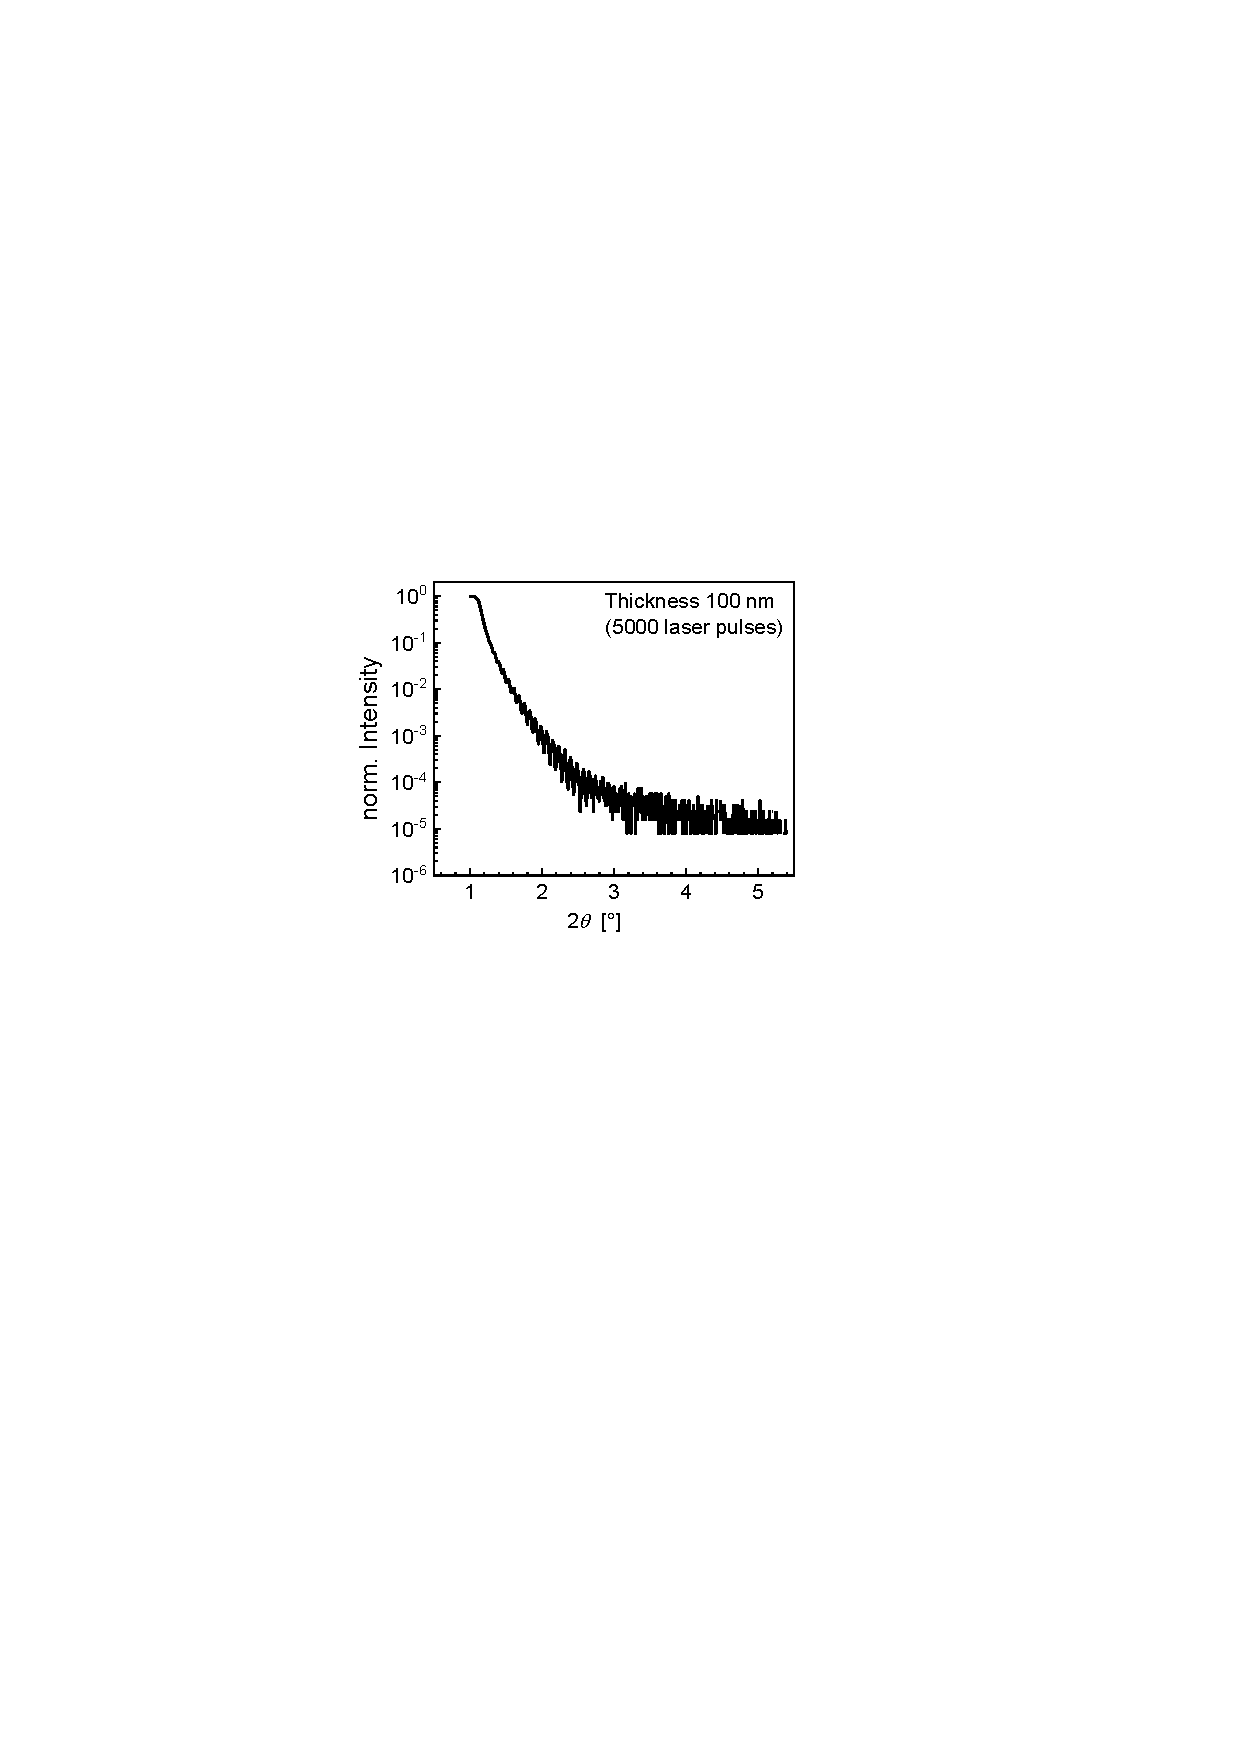
\includegraphics[width=0.6\textwidth]{content/pics/kiessig_oscillation.pdf}
    \caption{Kiessig Oszillationen an einem Multischichtsystem. Die Oszillationen sind das Resulatat von Interferenzen der reflektieren und eintreffenden %
    Strahlung \cite{kiessig_oscillation}.}
    \label{fig:kiessig_oscillation}
\end{figure}

Die Schichtdicke $d$ des Multischichtsystems kann mithilfe der Kiessig Oszillationen bestimmt werden. Dafür wird der Zusammenhang

\begin{equation}
    d = \frac{\lambda}{2\symup{\Delta}\alpha}
    \label{eq:Schichtdicke}
\end{equation}

zwischen der Wellenlänge $\lambda$ der Röntgenstrahlung und dem Abstand $\symup{\Delta}\alpha$ zweier Extrema mit gleichem Vorzeichen verwendet.

Verfügt ein Material über mehr als zwei Schichten, überlagern sich die Oszillationen. Mithilfe des so genannten Parrat-Algorithmus können erneut die Schichtdicken berechnet werden.
Dafür wird die Rekursionsformel
\begin{equation}
    X_{\symup{j}} = \frac{R_{\symup{j}}}{T_{\symup{j}}} = \symup{e}^{-2\symup{i}k_{\symup{z}}z_{\symup{j}}}\frac{r_{\symup{j,j+1}}+X_{\symup{j+1}}\symup{e}^{2\symup{i}k_{\symup{z,j+1}}z_{\symup{j}}}}%
    {1+r_{\symup{j,j+1}}X_{\symup{j+1}}\symup{e}^{2\symup{i}k_{\symup{z,j+1}}z_{\symup{j}}}} % ???????????
    \label{eq:Parrat}
\end{equation}
verwendet. Hier bezeichnet $r_{\symup{j,j+1}}$ die Fresnelreflektivität der j-ten Grenzschicht und $k_{\symup{z,j}}$ die z-Komponente des Wellenvektors $\vec{k}$ der j-ten Schicht.
Dabei gilt
\begin{equation*}
    k_{\symup{z,j}} = \sqrt{n_{\symup{j}}^2 -\cos^2 \alpha}.
\end{equation*}
Die erste und letzte Schicht werden als unendlich angenommen und somit wird dort nicht weiter reflektiert, was den Startwert der Rekursion auf $R_{\symup{N+1}} = X_{\symup{N+1}} = 0$ setzt.

Damit der Parrat-Algorithmus nicht nur für glatte, sondern auch für raue Oberflächen verwendet werden kann, wird eine \textit{root-mean-square}-Rauigkeit 
\begin{equation*}
    \sigma_{\symup{j}}^2 = \int (z-z_{\symup{j}})^2 P_{\symup{j}}\symup{d}z
\end{equation*}
eingeführt. Dafür wird die Position in der j-ten Schicht $z_{\symup{j}}$ sowie die Wahrscheinlichkeit $P_{\symup{j}}$, dass diese sich in einem Intervall 
$[z_{\symup{j}}+z, z_{\symup{j}}+z+\symup{d}z]$ befindet, benötigt. Die Wahrscheinlichkeitsverteilung wird als Gaußverteilung angenommen.
Mithilfe der \textit{root-mean-square}-Rauigkeit ergeben sich die modifizierte, rekursive Fresnelgleichungen

\begin{align}
    \label{eqn:r_korrigiert}
    r´_{\symup{j,j+1}} &= r_{\symup{j}}\symup{e}^{-2k_{\symup{z,j}}k_{\symup{z,j+1}}\sigma_{\symup{j}}^2} & t´_{\symup{j,j+1}} &= t_{\symup{j,j+1}}\symup{e}^{\frac{(k_{\symup{z,j}}-k_{\symup{z,j+1}})^2\sigma_{\symup{j}}^2}{2}}.
\end{align}
Diese können erneut in den Parrat-Algorithmus \eqref{eq:Parrat} eingesetzt werden, sodass die korrigierten Schichtdicken bestimmt werden können.

\subsection{Korrektur um einen Geometriefaktor}
Wenn die Röntgenstrahlung in einem kleinen Winkel auf die Probe trifft, beleuchet die Strahlung nicht die gesamte Probe. Eine Skizze zur Veranschaulichung dieses Sachverhalts ist in
\autoref{fig:Geometriewinkel} gegeben. Für Winkel unterhalb eines Grenzwinkels $\alpha_{\symup{g}}$ muss daher ein Korrekturfaktor $G$ eingeführt werden.
Der Grenzwinkel $\alpha_{\symup{g}}$ berechnet sich aus der Länge der Probe $D$ und der Strahlbreite der Röntgenstrahlung $d_0$ zu
\begin{equation}
    \label{eqn:a_g}
    \alpha_{\symup{g}} = \arcsin \left(\frac{d_0}{D}\right).
\end{equation}
Für den Geometriefaktor $G$ gilt
\begin{equation}
    G = 
    \begin{cases*}
        \frac{D\sin \alpha}{d_0}  & für $\alpha < \alpha_{\symup{g}}$ \\
        1 & sonst.
    \end{cases*}
    \label{eq:Geometriefaktor}
\end{equation}

\begin{figure}
    \centering
    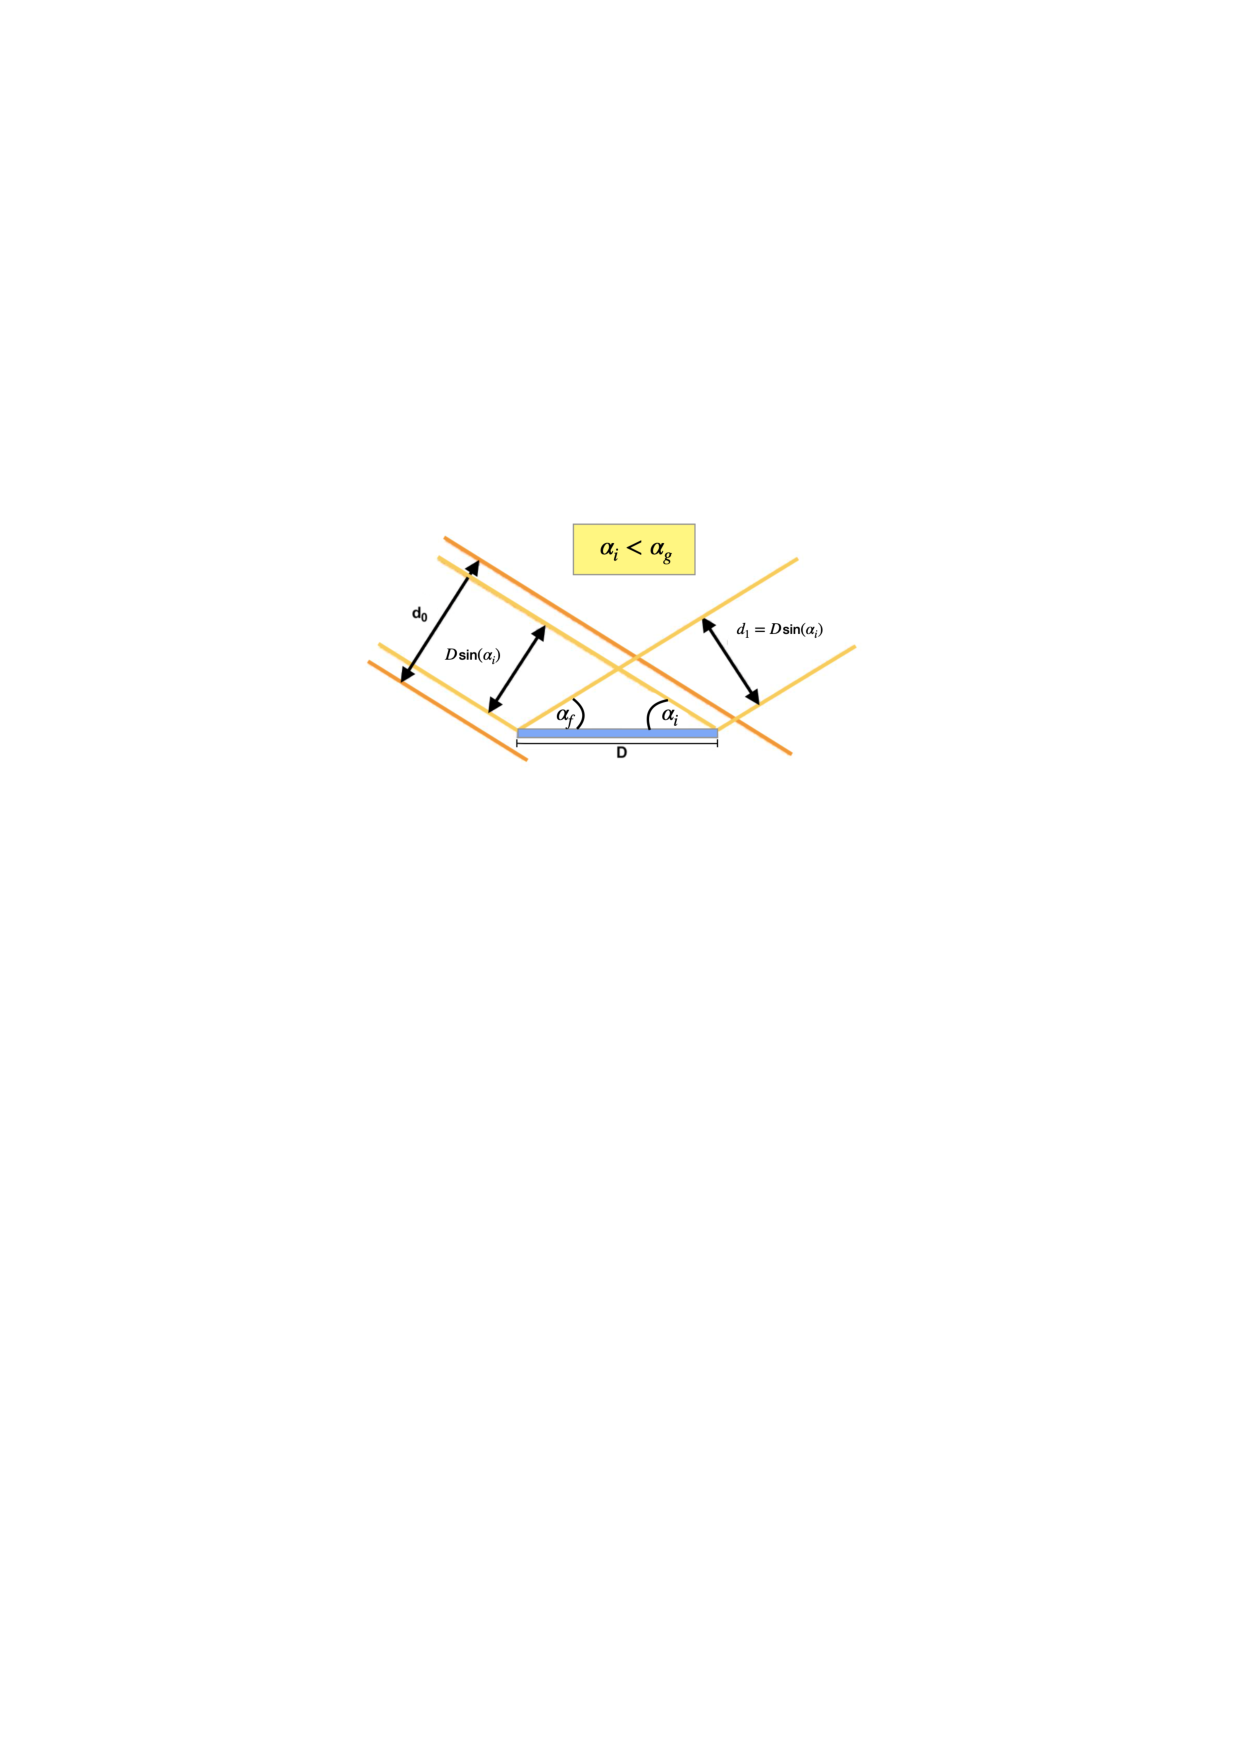
\includegraphics{content/pics/Geometriewinkel.pdf}
    \caption{Veranschaulichung der verwendeten Größen zu der Einführung des Geometriefaktors $G$ \cite{V44}.}
    \label{fig:Geometriewinkel}
\end{figure}